\documentclass[12pt]{standalone}

% main document, called main.tex \usepackage{tikz}
% \usetikzlibrary{external}
% \tikzexternalize % activate!

\usepackage{tikz}
\usetikzlibrary{decorations.markings}


\begin{document}
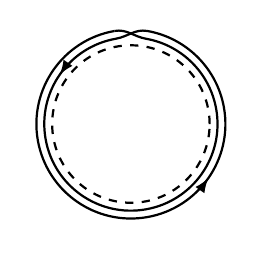
\begin{tikzpicture}

% Draws the dashed line
\draw[
    thick,
    dashed,
    ] 
    (0,0) circle (1cm);

% Inner points
\coordinate (A) at (-0.19101299543362335, 1.0832885283134288);
\coordinate (B) at (0.19101299543362346, 1.0832885283134288);

% Outer points
\coordinate (C) at (-0.20837781320031637, 1.1817693036146495);
\coordinate (D) at (0.20837781320031648, 1.1817693036146495);

% Inner circle
\path[
    draw,
    thick,
    decoration={markings, mark=at position 0.125 with {\arrow[black]{latex}}},
    postaction={decorate}
    ]
    (A) arc (100:440:1.1) to[out=170, in=10] (C);

% Inner path
\path[
    draw,
    thick,
    decoration={markings, mark=at position 0.625 with {\arrow[black]{latex}}},
    postaction={decorate}
    ]
    (C) arc (100:440:1.2) to[out=170, in=10] (A);

\end{tikzpicture}
\end{document}